\documentclass{article}

\usepackage{float}
\usepackage{graphicx}
\usepackage{caption}
\usepackage{subcaption}

\title{DeepHEC: Deep Reinforcement Learning for robotic Hand-Eye Coordination}
\author{Hayden Sampson $<$sampsoh@edgehill.ac.uk$>$}
\date{2021}


\begin{document}
\maketitle

\begin{abstract}
Reinforcement Learning has proven to be an effective approach for solving 	Artificial Intelligence (AI) tasks over recent years. Utilisation of Deep Neural Networks for Deep Reinforcement Learning (DRL) has led to state-of-the-art methods and results for tasks relating to game play and robotic control/movement. Here, we explore the effectiveness of DRL for robotic control that involves visual pixel image inputs and arm control action output for a task concerning grasping a diverse range of objects from a table. This research extends current work by including methods to improve data efficiency of algorithms, such as Hindsight Experience and introducing the use of Attention Mechanisms to evaluate performance on such as task and environment. Our results show... indicating...
\end{abstract}
\section{Introduction}
The use of reinforcement learning methods to perform and succeed in certain tasks and increased significantly over recent years. Initial success using reinforcement learning was presented in its' ability to learn how to solve certain simple tasks such as balancing an inverted pendulum [reference] or learning to land a lunar lander between two flags [reference]. This opened up opportunities to explore the effectiveness of reinforcement learning for tasks requiring pixel image input by playing a range of Atari games [reference]. Such study introduced more complex environments for reinforcement learning, such as those including much larger state and action spaces. Because of this, standard reinforcement learning was not viable for effective and efficient performance. Deep Neural Networks (DNN) solved this issue, with combination of reinforcement learning that introduced Deep Reinforcement Learning methods to allow agents to outperform human level on a number of Atari games [reference]. Since, there has been an exponential increase in work and study to further improve these methods and to succeed in a variety of other tasks that an agent could solve. One such problem includes those tasks related to robotic arm control and movement, including grasping, inserting, pick-and-place and sliding.
\\
Although there has been a lot of good work and study into the development of DRL models for these tasks [references], there has been yet to find an appropriate solution to generating high performing data efficient models. Many DRL methods require a large amount of data, and therefore time, in order to be successful at the given task, especially for robotic arm control. Because of this, there is ample opportunity for exploration into developing DRL models that are much more sample efficient and can train much faster whilst providing a high level performance. In this case, we have explored two such methods: Episodic Self Imitation Learning (ESIL) [reference] and Attention Mechanisms [reference].

\section{Literature Review}
There has been extensive research in studies regarding the areas in Deep Reinforcement Learning, including specific focus on the problems of robotic arm movement and grasping. DeepMind’s Atari [Mnih2013] first brought into the light the effectiveness of using deep reinforcement learning and ‘Deep Q Networks’ (DQN) for outperforming human performance over a range of Atari games. The novelty of this study showed how these algorithms can make use of graphical pixel images as state inputs to output appropriate actions in the environment. What was also impressive was the breakaway from model-based methods to model-free, where a network could show similar high-scoring performances when trained on a variety of different games.
\\\\
In terms specific to robotic arm control, Google Brain [Quil2018] has explored the subject through a comparative implementation of a number of well-known off-policy learning methods. This presented a good starting place for analysing algorithmic performances for such tasks, and has proven to be highly influential for the motivation behind this proposed research. Where the study lacks is in the comparison and analysis of on-policy methods such as TRPO [Schul2015] and PPO [Schul2017] learning, which have also been proven through other studies to be effective for robotic control [Mahmood2018]. As well as this, the study has omitted methods that have been proven to improve algorithm performance and sample efficiency, such as Prioritised Experience Replay [Schaul2016] or Hindsight Experience Replay [Andry2018], that also prove to be highly effective for robotic arm environments.
\\\\
Further research [Blake2020] explores increasing efficiency through attention models, with the aim of reducing the visual field of an agent to only focus on the important aspects of an input image, in order to reduce feature state space and dimensionality.


\section{Background}
\subsection{Deep Reinforcement Learning}
Generally, the standard reinforcement learning is concerned with producing an agent that learns how to take appropriate actions within an environment to gather rewards and succeed in a certain task. An indicator that a task has been achieved successfully is the amount of reward an agent will receive, therefore an agent will learn to act in whichever way will allow it to gain the most reward. Agents will make observations of the current state of the environment and make decisions on how to act based on this, producing state-action transition pairs. How an agent makes a decision on what action to take is called the agent’s policy. Taking an action causes the environment to change and update state as well as giving the agent some reward. The agent can then make a new observation on the updated state and take a new action.

\begin{figure}[H]
\centering
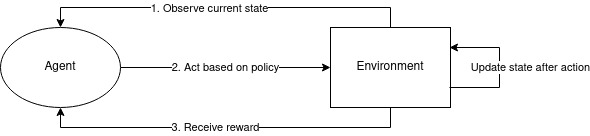
\includegraphics[scale=0.5]{RLCycle}
\caption{Reinforcement Learning Cycle}
\label{rlcyclefig}
\end{figure}

This cycle is repeated for T timesteps until the environment reaches its termination state, with the states between and including the initial state and final state defining an episode. The learning process therefore involves an agent figuring out which actions to take that will eventually lead to the greatest reward at the end of an episode (cumulative reward).

The standard reinforcement learning approaches assume a discrete state and action space and hence, suffer from the curse-of-dimensionality problem which simply states the computational complexity increases exponentially with increasing dimensions of state and action space. The problem of discrete state space can be solved by using deep networks that can take continuous values as inputs including images. In other words, Deep Reinforcement Learning (DRL) methods use deep networks to overcome some of the limitations of standard reinforcement learning. These methods can be broadly divided into two categories: model-based and model-free methods. We are primarily interested in the model-free methods, that do not act based on their knowledge or estimation of the environment, but solely on the observation of the current state of the environment arrived at by using a given policy. These model-free methods can be further divided into two sub-categories depending on how the agents learn, namely policy-based and value-based learning. Value-based methods estimate a Q-value (cumulative future reward) to every state-action pair by using a Q-function Q(s, a) and then select an action which gives a maximum Q value at a given state.  So, in essence, value-based learning is concerned with estimating or approximating the Q-function. On the other hand, policy-based learning aims at estimating  a policy  directly without estimating the Q function. The policy parameters are updated to maximize or minimize a given objective function.  For instance, policy gradient methods update the policy parameters by applying gradient ascent to maximize a given objective function. The advantage of using policy-based learning for this research problem is that it can be much more easily applied to agents with a continuous action space, as an action is being directly outputted from the network, rather than a Q-value for each possible action available. Another categorization can be made based on how the agents are trained. The on-policy methods train the agent using data generated using its current policy. This is an online approach where the agent is learning while doing its  job. In contrast, off-policy methods use a set of experience for training which are generated by a different policy than the one currently being  used by the agent. It is possible to combine these two approaches in the form of an Actor-Critic algorithm  [KonTsi2000]  that employ a policy-based method to choose an action, with a value-based method to assign values to specific state-action pairs that critique how good that action was. Actor-Critic methods will form the underlying architecture used in this research.

\subsection{Proximal Policy Optimisation}
Proximal Policy Optimisation (PPO) is an on-policy algorithm first introduced by [reference], that sought to improve performance of Trust Region Policy Optimisation (TRPO) [reference], whilst also simplifying implementation and increasing sample efficiency. The idea behind the algorithm is simple, limit the magnitude in which the policy is updated after each training step to erase the possibility of the gradient update stepping too far. Doing so controls the stability of the training process. The step control can be implemented through two methods: clipping or use of a KL penalty. For clipping, there is simply a value $\epsilon$ that act as the upper and lower boundaries for the step magnitude. Alternatively, a KL Divergence method can be used to describe the similarity between two probability distributions and constrains the objective step function based on this. For this research, PPO-Clipping has been implemented.
\subsection{Episodic Self Imitation Learning}
In regards to improving DRL methods to be more sample efficient, a lot of promise has been presented through the use of Hindsight Experience Replay (HER) [reference]. This works more specifically for environments with sparse rewards, such as the one explored in this study. Originally, HER as a method had only been applicable to use with off-policy methods, such as Deep Deterministic Policy Gradient (DDPG) [reference]. This is because the hindsight experience used in training is collected from a memory buffer that contained samples from all past policies. In order to make hindsight experience compatible with on-policy methods, Episodic Self Imitation Learnig (ESIL) [reference] was introduced which combined aspects of Self Imitation Learning (SIL) and HER to allow hindsight experience collected from the current policy only to be used in training.
\subsection{Attention Mechanisms}
Attention Mechanisms were first introduced in [reference] and were inspired by the way humans perceive and focus on certain aspects of our vision to take in the most important information for whatever task we are undergoing. Two main types of attention were realised, bottom-up saliency attention and top-down task relevant attention (or vice versa, check this). Saliency attention comes from the idea of what grabs our attention that is in our field of vision, in other words what is the most visually interesting thing that demands attention. Task related attention comes from the idea of what we need to pay attention to in order to fulfill a task, for example throwing a ball into a hoop, we would likely focus most of our attention on the hoop.

\section{Experiments}
\subsection{Model Architecture and Approach}
In this research, we  primarily make use of actor-critic models as shown in Figure \ref{acfig} below. In this model, we have two separate networks - one for estimating the policy  required for generating the necessary action and the other for approximating the Q function or the value function  that can be used to evaluate the goodness of the action taken. These two networks are updated iteratively to find the optimal policy for a given problem by maximizing the total cumulative reward . This architecture provides flexibility in selecting different architectures and algorithms for each of the actor and critic modules independently. Each of the actor and critic models will use a deep neural network (DNN) to estimate action and value from the input state information. The environment provides the reward  and the next state  for a given state-action pair. The goal of learning will be to update parameters and so that certain objective cost functions are either maximized and minimized. 

\begin{figure}[H]
\centering
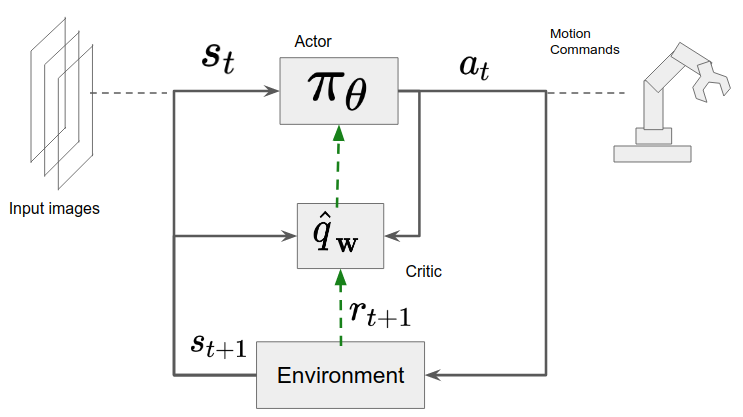
\includegraphics[scale=0.4]{actor-critic}
\caption{Actor-Critic Architecture}
\label{acfig}
\end{figure}

\subsubsection{Simulation Environment}
Our objective is to develop, test and validate new deep reinforcement learning algorithms for solving robotic problems. In this regard, we have selected OpenAI/Gym’s KukaCam [PyBullet2017] as our simulation environment. Some of the screenshots for this environment is shown in Figure \ref{envfig}. In this environment, a 6DoF Kuka robotic arm is expected to pick up different kinds of objects from the tray kept on the table based on the input images seen by an overhead camera. The view of the camera is shown in the top left corner of each image. This image along with the current joint values of the robotic arm (robot pose) forms the current ‘state’ of the environment. The agent is rewarded a value of 1 whenever the robot successfully picks up an item from the tray, otherwise the rewarded value is 0. Each episode consists of a series of robot movements attempting to pick an item. The objective is to pick the item successfully based on an input image obtained from the overhead camera.

\begin{figure}[H]
\centering
\begin{subfigure}{.5\textwidth}
  \centering
  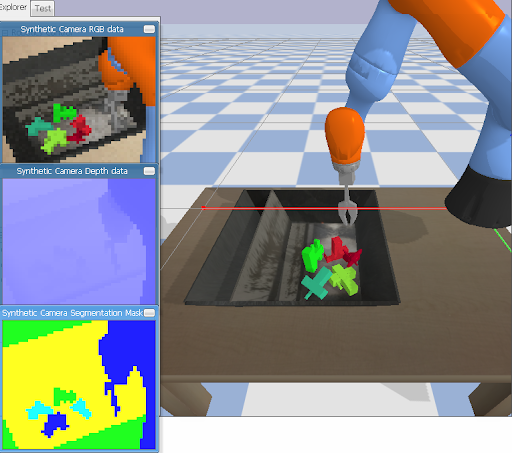
\includegraphics[scale=0.32]{kuka_env1}
\end{subfigure}%
\begin{subfigure}{.5\textwidth}
  \centering
  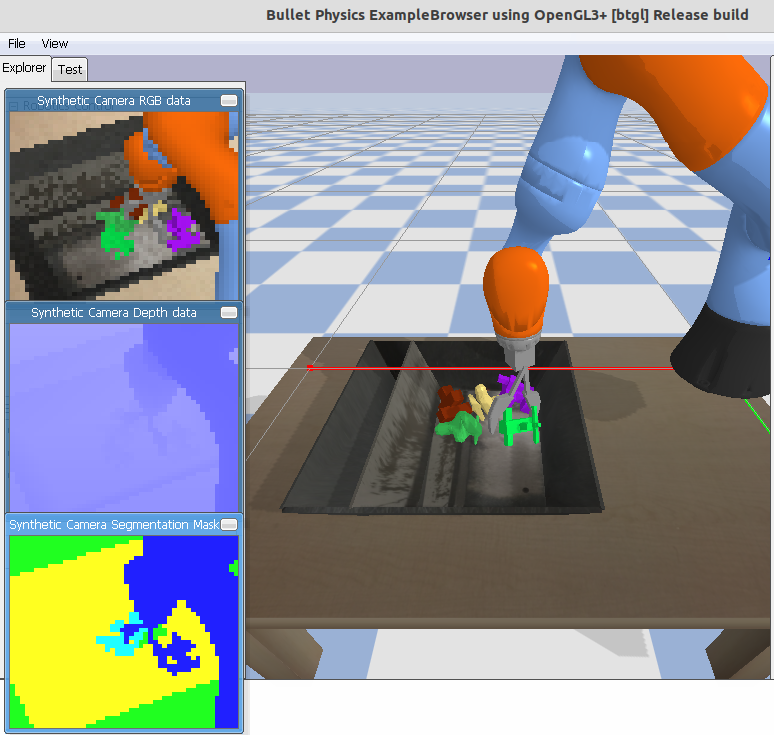
\includegraphics[scale=0.20]{kuka}
\end{subfigure}
\caption{Pybullet KukaCam Diverse Object Environment}
\label{envfig}
\end{figure}

\subsubsection{Deep Neural Net Design}

\begin{figure}[H]
\centering
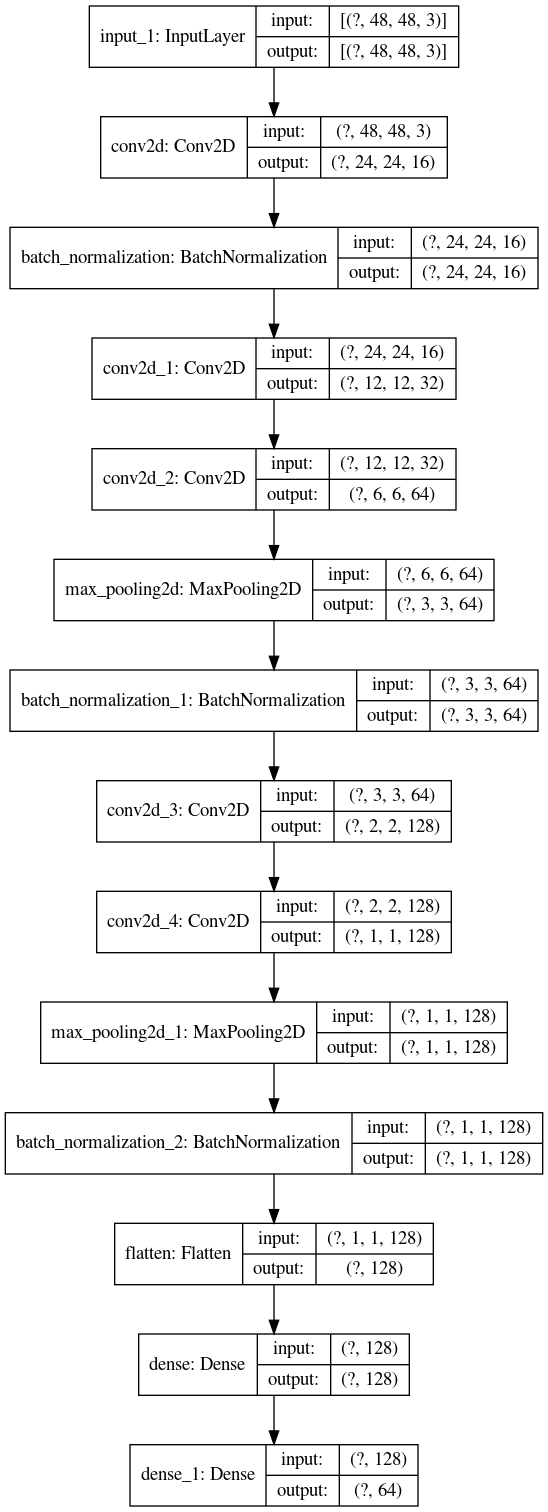
\includegraphics[scale=0.3]{feature_net}
\caption{Convolutional Neural Network}
\label{cnnfig}
\end{figure}

\subsection{Hyperparameters and Setup}
\begin{table}[H]
\centering
\begin{tabular}{|l|l|}
\hline
\textbf{Hyper-parameter}  & \textbf{Value} \\ \hline
Clipping value $\epsilon$ & 0.07           \\ \hline
Actor Learning rate       & 0.0003         \\ \hline
Critic Learning rate      & 0.0002         \\ \hline
Epochs                    & 10             \\ \hline
Season time steps         & 1024           \\ \hline
Batch size                & 128            \\ \hline
Gamma $\gamma$            & 0.7            \\ \hline
Lambda $\lambda$          & 0.993          \\ \hline
\end{tabular}
\caption{Hyperparameters}
\label{hyperparams}
\end{table}
\subsection{Results}

\section{Discussions and Conclusion}

\section{References}
\end{document}